\chapter{IMPLEMENTATION DETAILS}
\section{Model Implementation}
\vspace{10pt} % Adjust the value as needed

\subsection{Preprocessing}
In our project, we utilized data from EVERESTner to classify Named Entities within sentences, encompassing 20,000 annotated sentences with labels such as B-Person, I-Person, B-Organization, I-Organization, B-Location, and I-Location. Originally in TXT format, this dataset was sourced from a GitHub repository. Concurrently, for model development, we drew insights from the WikiANN dataset, where meticulous data cleaning and preprocessing were imperative for training our SABDA-NER model. Each row in the WikiANN dataset contained 100 Nepali language sentences, and we seamlessly integrated this dataset into our training process.\\
\\
To further evaluate the model, we curated our own dataset for testing purposes, consisting of 1,700 manually annotated rows. This dataset serves to gauge the model's performance on novel and unseen data, allowing us to assess its generalization capabilities beyond the training data from EVERESTner and WikiANN.\\
\\
In the preprocessing phase, we initially converted our EVERESTner data into a CSV file, adhering to the specified annotation format. Subsequently, this data was transformed into a JSON file, aligning with the WikiANN structure, necessitating the use of "token\_set" and "ner\_tags" with numerical entity labels. String labels were replaced with numerical values, and after removing unnecessary columns, the formatted data was saved as a JSON file in our Google Drive.

\subsection{Model Description}
We developed our model using Google Colaboratory, leveraging the T4 GPU hardware accelerator. To load our data into Colab, we imported datasets from Hugging Face. Subsequently, we installed and imported the BERT tokenizer to tokenize Nepali language sentences and words. Further, we installed PyTorch. For evaluating the model's performance, we imported Seqeval to obtain score matrices, including accuracies and F1 scores.\\
\\
Our model was trained on the BERT-based-multilingual-cased architecture, chosen for its versatility across multiple languages. This model is widely used and reliable for custom data. Additionally, we incorporated W\&B (Weights \& Biases) for tracking machine learning work and training procedures, providing visualizations of model performance and scores.\\



\begin{figure}[H]
\centering
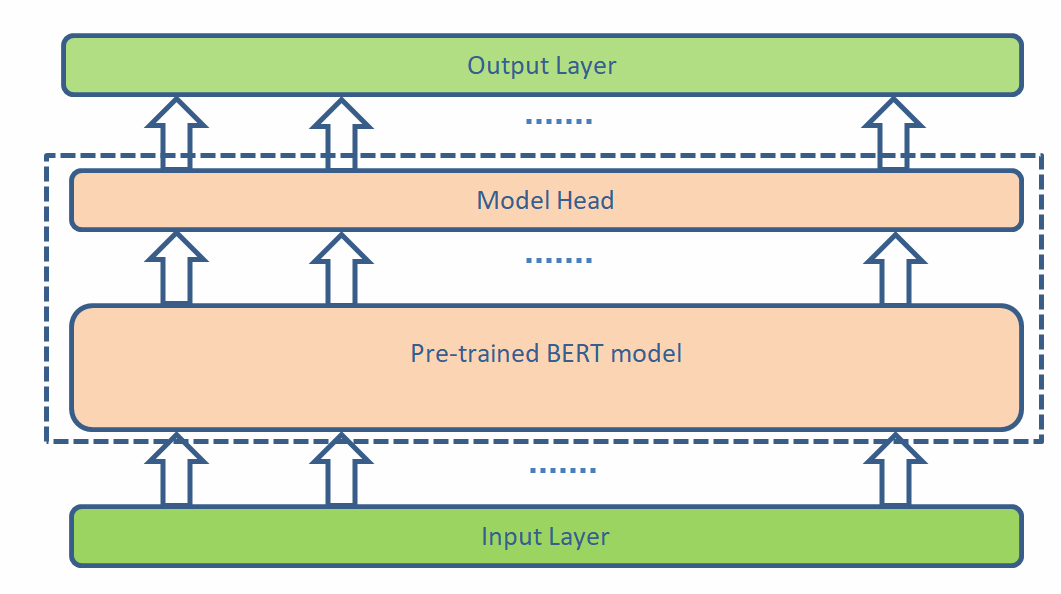
\includegraphics [scale=0.6]{img/Graphics/Model training Information.png}
\caption[Model training Information]{ Model training Information \textit{(Source: \href{https://www.analyticsvidhya.com/blog/2022/09/fine-tuning-bert-with-masked-language-modeling/}{Analytics Bidhya, 2024})}}
% \label{fig:DisplaCy.png}

\end{figure}






  
We saved our model on Google Drive, enabling anyone with access to the model location to import and test results. Currently, testing involves manual sentence insertion, and we plan to extend this to test the entire dataset of 1,700 sentences at once for comprehensive evaluation. Initial scores are promising, and our next step is deploying the model on our website by uploading it to Hugging Face.

\subsection{FastAPI}

FASTAPI emerges as a crucial tool for deploying our NER model on the website. With FASTAPI, users can seamlessly interact with our model through the website's interface, enabling them to input sentences or links for information extraction via web scraping. This framework facilitates the smooth transfer of data from the user interface to the model, ensuring efficient processing of named entity classifications. The use of FASTAPI enhances the overall user experience, making it easy and reliable to obtain accurate results.

\subsection{Web Scraping}
Web scraping is a technique used to extract information from websites. It involves automatically fetching and parsing web page content to gather data, such as text, images, or links. Think of it as pulling useful information from a website's pages, making it accessible for various purposes, like analysis or integration into other applications. However, it's important to note that web scraping should be done ethically and in compliance with the website's terms of service.\\
\\
When deploying our model on the website, users can visit the site and input their sentences directly. Additionally, they have the option to insert a link on our website, allowing us to perform web scraping on the provided link. Our objective is to extract named entities, including persons, locations, and organizations, using our website. To access the web scraping procedure on the provided link, users need to navigate to the designated section on our website. Once initiated, the system will read all entities from the link and display the results on the screen of our website.

\section{Implementation of Bidirectional Encoder Representations from Transformers (BERT)}

\vspace{20pt}

 \begin{figure}[H]
\centering
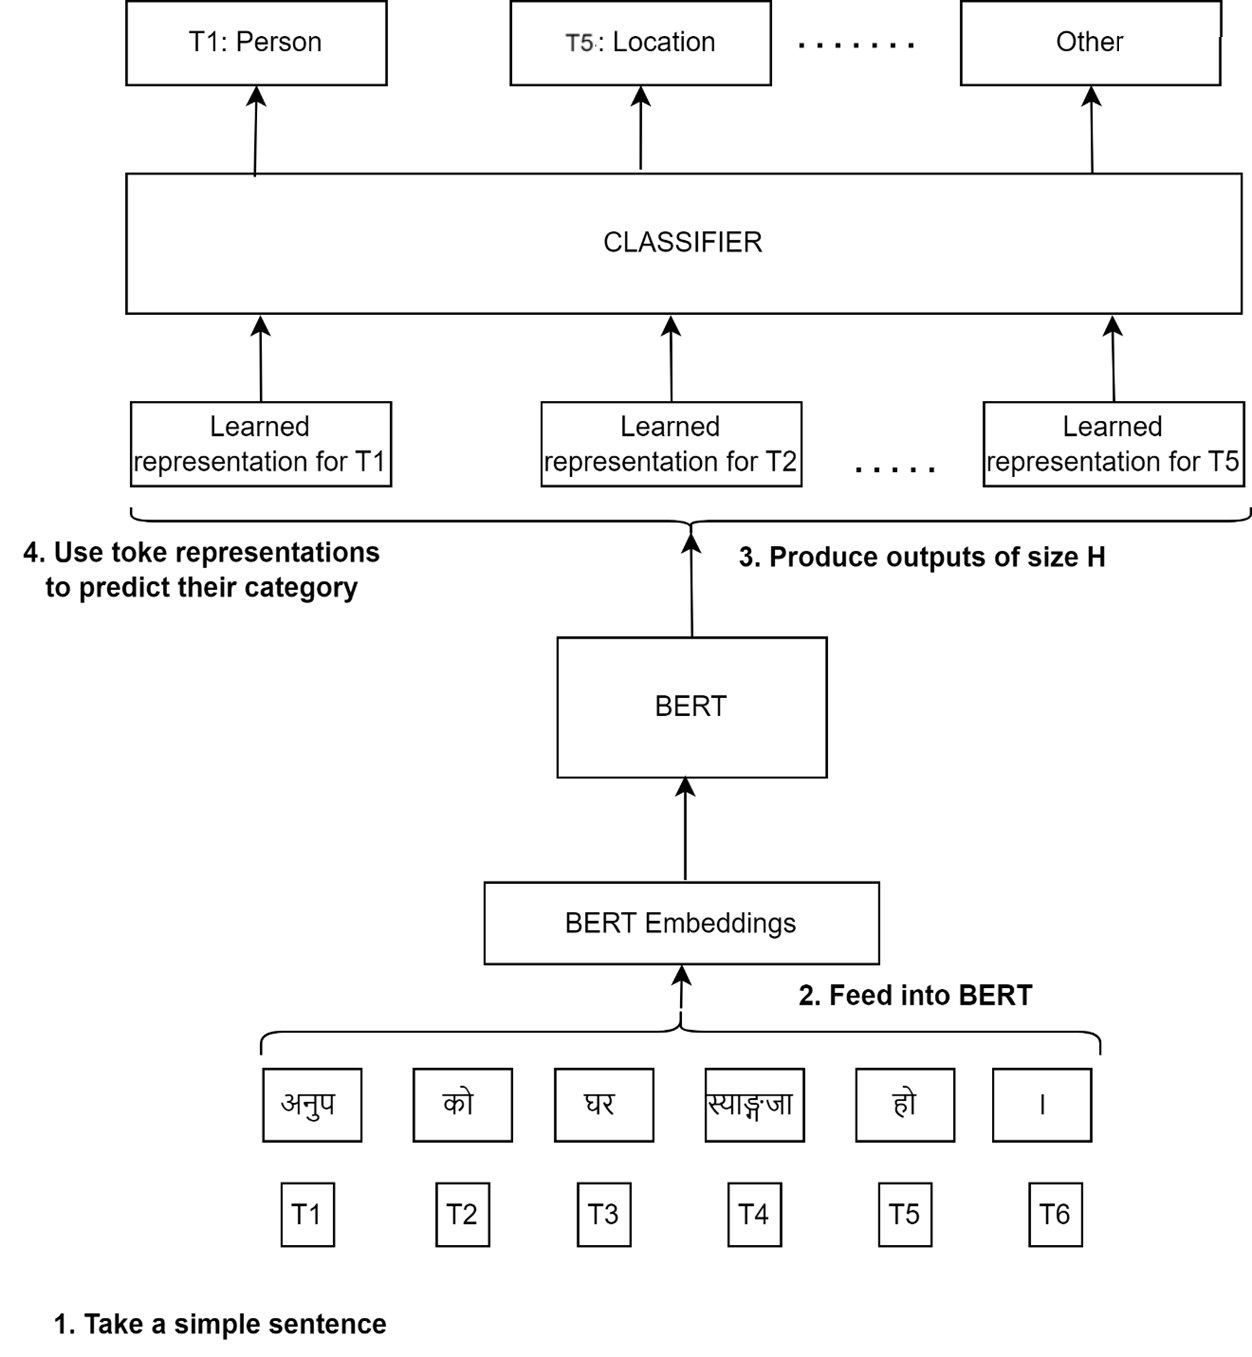
\includegraphics[width=1\textwidth]{img/systemBlock-etc/System Block diagram.png}
\caption[ System Block diagram]{ System Block diagram}

\end{figure}


 \subsubsection {Input Stage}
Input Text: The system takes raw text as input, which is the text to be analyzed for named entities.
\subsubsection{Intermediate Stages}
Tokenization and Embedding Layer: This stage involves tokenizing the input text into individual tokens and converting them into numerical embeddings using BERT's vocabulary. This layer also includes adding segment embeddings and positional encodings.
\subsubsection{Multi-Head Self-Attention and Feedforward Layers}
The token embeddings go through multiple layers of multi-head self-attention mechanisms and feedforward neural networks. This helps the model capture contextual relationships and create rich representations of the input tokens.
\subsubsection{NER Classification Layers} 
On top of the final hidden states, additional classification layers are added. These layers include fully connected networks followed by softmax activation. These layers predict the probability of each token belonging to different named entity classes (e.g., person, organization, location).
\subsubsection{Output Stage}
NER Predictions: The output of the NER classification layers provides predictions for each token's named entity label. Common labels include "B-PER" (beginning of a person entity), "I-PER" (inside a person entity), "B-ORG" (beginning of an organization entity), and so on.


\newpage
\section{Description of Algorithm}
\vspace{10pt} % Adjust the value as needed
\subsection{Entities Set} 
Natural Language Processing (NLP)’s named entity recognition (NER) sub-component seeks to identify the textual existence of entities that fall under a predetermined set of categories, such as “PERSON”, “LOCATION”, and “ORGANIZATION”.

\subsection{Annotation Guidelines}
We developed detailed annotation guidelines that cover entity types, variations, and potential challenges specific to the Nepali language. These guidelines will ensure consistent labeling during the annotation process.\\

 
\begin{table}[H]
  
\caption{ Annotation Guidelines}
\label{tab:  Annotation Guidelines}
    \centering
    
    \begin{tabular}{|c|c|c|}
        % \hline
        % Column 1 & Column 2 & Column 3 \\
        % \hline
        % Row 1, Cell 1 & Row 1, Cell 2 & Row 1, Cell 3 \\
        % Row 2, Cell 1 & Row 2, Cell 2 & Row 2, Cell 3 \\
        % \hline
    \end{tabular}
    
    
\end{table}
\begin{figure}[H]
\centering
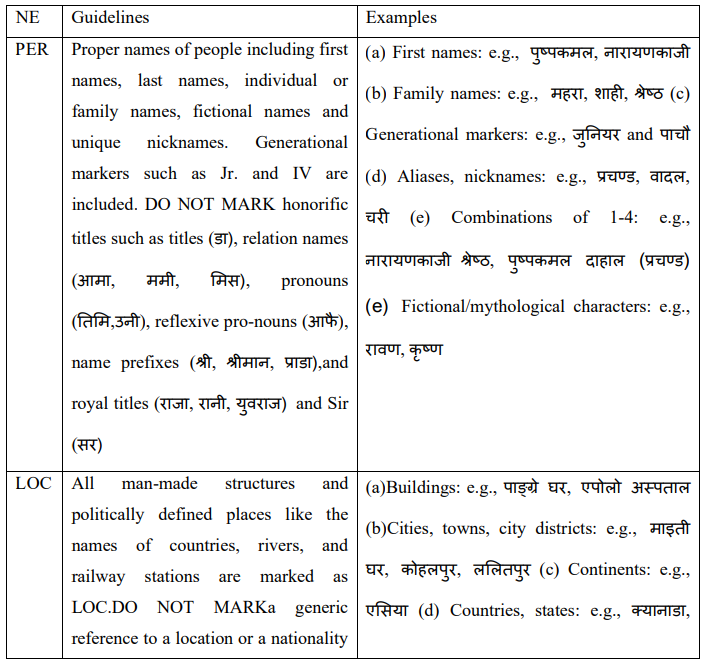
\includegraphics [scale=1.2]{img/Graphics/Annotation Guidelines1.png}
% \caption[ Annotation Guidelines]{ Annotation Guidelines}
% \label{fig:DisplaCy.png}

\end{figure}
\begin{figure}[H]
\centering
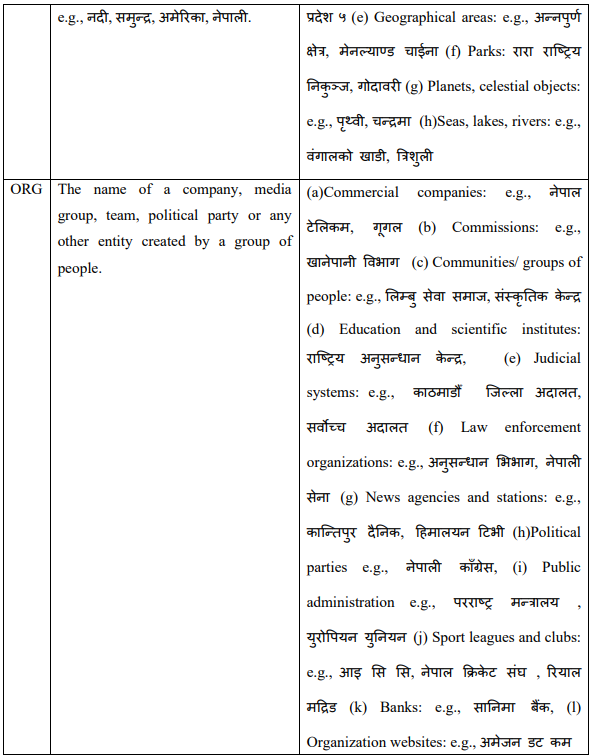
\includegraphics [scale=1.4]{img/Graphics/Annotation Guidelines2.png}
% \caption[ Annotation Guidelines]{ Annotation Guidelines}
% \label{fig:DisplaCy.png}

\end{figure}



 
 
\subsection{Model Selection}
We fine-tuned pre-trained models that was trained for multi-lingual, the BERT-based-multilingual-cased model. To tailor it for Nepali, we began with a pre-trained model for a related language and fine-tuned it using our datasets.

\subsection{Data Splitting}
Splitting of annotated dataset into training, validation, and testing sets. A common split is 80-20, where 80\% of the data is used for training, and the rest is for validation, and we prepare few datasets to test the model.

\subsection{Fine Tuning}
As we utilized a pre-trained model, we proceeded to fine-tune it using our annotated Nepali dataset. Following the structure outlined in WikiANN, we tokenized the dataset into two sets—one for tokens and the other for NER tags. To adhere to the required format of .json files, we converted our annotated and cleaned dataset into train.json and validate.json files. These files were then used to train the model and validate its predictions.

\subsection{Model Evaluation}
We assessed our trained/fine-tuned model on the validation and testing datasets, employing metrics such as precision, recall, and F1-score. The model exhibited promising results, achieving an overall precision of approximately 0.98 across various validation and training datasets.

\subsection{Model Deployment}
We are working on deploying our model on a simple website, allowing users to enter the page, import their sentences, and extract the desired information.

\newpage
\section{Working Principle}
\vspace{10pt} % Adjust the value as needed
We have used News Corpus for preparing our dataset (Nepali News Corpus). News articles contain frequently used named entities. Articles have different domains like politics, sports, economics, art, society, and literature. The available corpus consists of text files. We used NLTK library to tokenize the text files. Preprocessing of data was done by removing punctuation marks and stop-words which helped to keep dataset clean. Later manual annotation was done to the dataset following the guidelines mentioned in data annotation.


 
\begin{figure}[H]
\centering
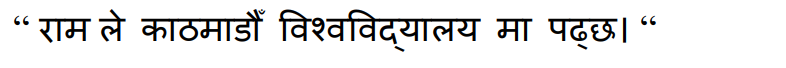
\includegraphics [scale=0.8]{img/workingPrinciple/ramle.png}
% \caption[ Annotation Guidelines]{ Annotation Guidelines}
% \label{fig:DisplaCy.png}

\end{figure}


The obtained tokens are annotated as follows:

  \begin{table}[H]
  
\caption{ Label Dataset with annotation guideline}
\label{tab:   Label Dataset with annotation guideline}
    \centering
    
    \begin{tabular}{|c|c|c|}
        % \hline
        % Column 1 & Column 2 & Column 3 \\
        % \hline
        % Row 1, Cell 1 & Row 1, Cell 2 & Row 1, Cell 3 \\
        % Row 2, Cell 1 & Row 2, Cell 2 & Row 2, Cell 3 \\
        % \hline
    \end{tabular}
    
    
\end{table}
 
\begin{figure}[H]
\centering
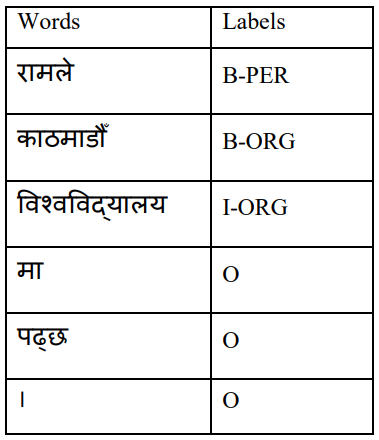
\includegraphics [scale=1]{img/workingPrinciple/ramle lebel.png}
% \caption[ Annotation Guidelines]{ Annotation Guidelines}
% \label{fig:DisplaCy.png}

\end{figure}
 
This data set is now all set for training. We have used the ‘Pytorch’ library for loading datasets to the training set into DataLoader. In PyTorch, when loading data using a DataLoader, it's crucial to convert text data into numbers for the model. This involves several steps for Named Entity Recognition (NER):
\newpage
\textbf{1.	Tokenization}: Split text into tokens.
           Tokenized Sentence:
           \begin{figure}[H]
\centering
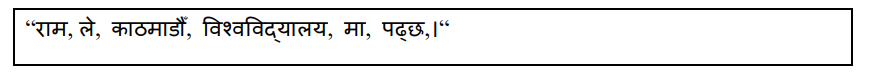
\includegraphics [scale=1]{img/workingPrinciple/ramle ku.png}
% \caption[ Annotation Guidelines]{ Annotation Guidelines}
% \label{fig:DisplaCy.png}

\end{figure}
 
           Labels:
           
\begin{figure}[H]
\centering
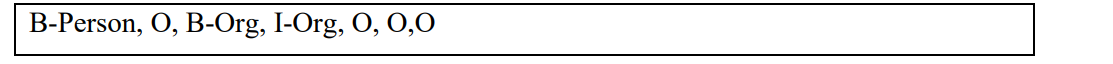
\includegraphics [scale=0.8]{img/workingPrinciple/org.png}
% \caption[ Annotation Guidelines]{ Annotation Guidelines}
% \label{fig:DisplaCy.png}

\end{figure}
 
\textbf{2.	Token-to-ID Mapping} : Convert tokens to numbers.
          
Tokenized Sentence:

\begin{figure}[H]
\centering
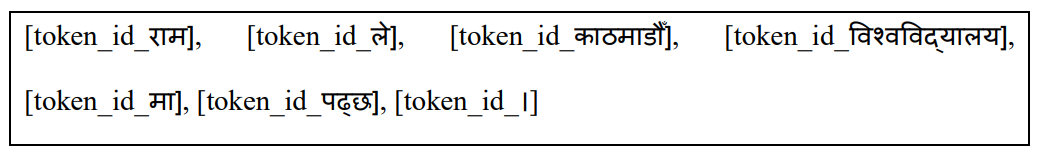
\includegraphics [scale=0.8]{img/workingPrinciple/token.png}
% \caption[ Annotation Guidelines]{ Annotation Guidelines}
% \label{fig:DisplaCy.png}

\end{figure}
 
\textbf{3.	Padding} : Make all sequences the same length.

\begin{figure}[H]
\centering
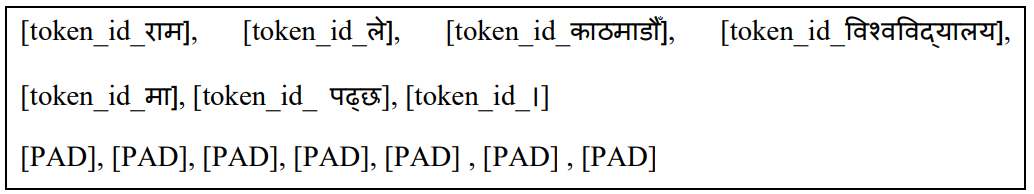
\includegraphics [scale=0.8]{img/workingPrinciple/token pad.png}
% \caption[ Annotation Guidelines]{ Annotation Guidelines}
% \label{fig:DisplaCy.png}

\end{figure}
 
\textbf{4.	Label Encoding} : Turn NER labels into numbers.
\begin{figure}[H]
\centering
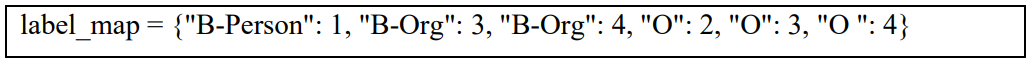
\includegraphics [scale=0.8]{img/workingPrinciple/lebelmap.png}
% \caption[ Annotation Guidelines]{ Annotation Guidelines}
% \label{fig:DisplaCy.png}

\end{figure}
 
 Encoded Labels:  
 \begin{figure}[H]
\centering
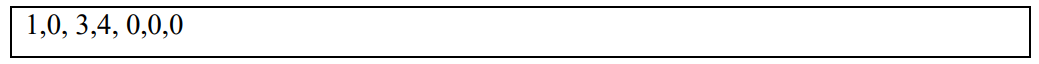
\includegraphics [scale=0.8]{img/workingPrinciple/0101.png}
% \caption[ Annotation Guidelines]{ Annotation Guidelines}
% \label{fig:DisplaCy.png}

\end{figure}
 
Data Loader of huggingface datasets enable efficient use of transformers as well as neural networks. They streamline data processing and enhance model training for tasks like NER. 
After properly loading our dataset in the DATA loader we will be using BERT-based-multilingual pre-trained model (Initial Phase) and also refer other models to train and fine-tune our model.

 

\section{Dataset Collection}

\begin{table}[H]
  
\caption{Data Set Stats}
\label{tab: Data Set Stats}
    \centering
    
    \begin{tabular}{|c|c|c|}
        % \hline
        % Column 1 & Column 2 & Column 3 \\
        % \hline
        % Row 1, Cell 1 & Row 1, Cell 2 & Row 1, Cell 3 \\
        % Row 2, Cell 1 & Row 2, Cell 2 & Row 2, Cell 3 \\
        % \hline
    \end{tabular}
    
    
\end{table}

\begin{figure}[H]
\centering
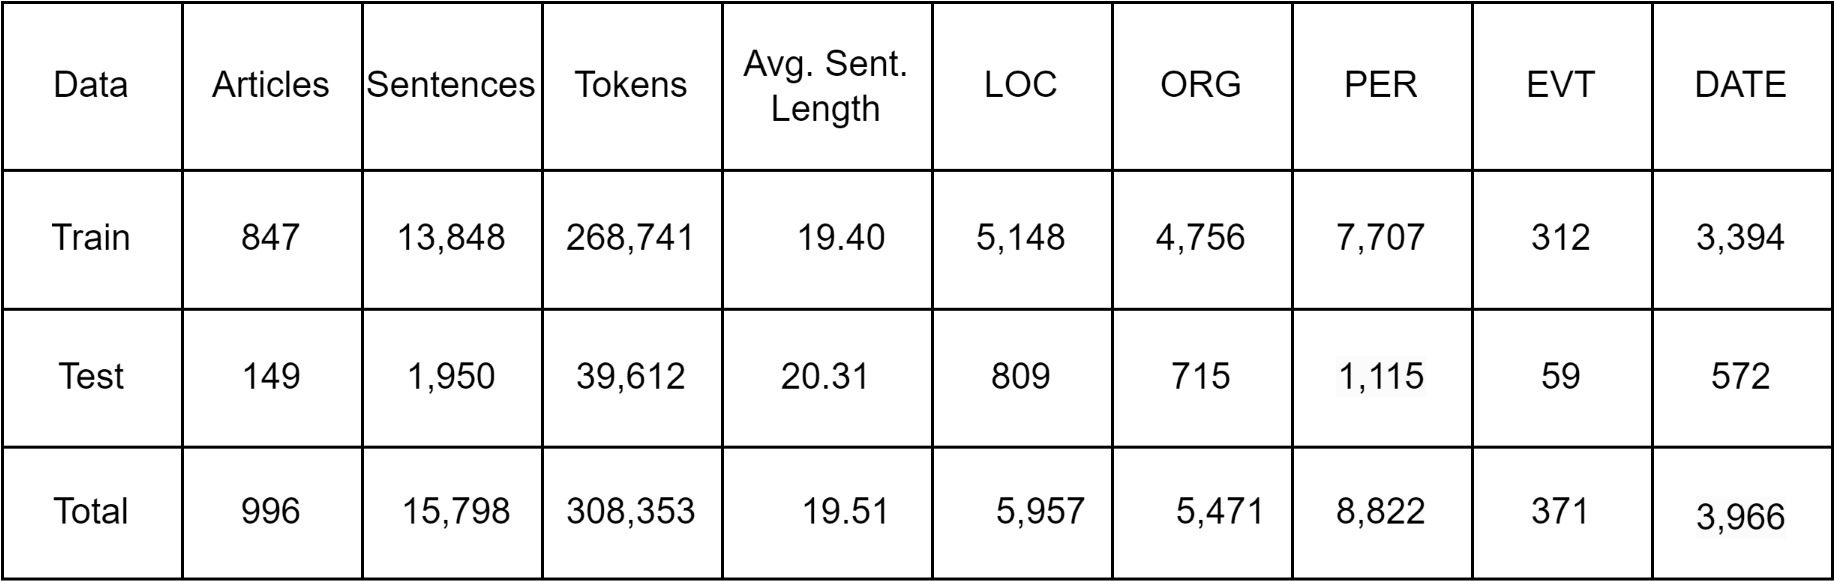
\includegraphics [scale=0.9]{img/Graphics/Data Set Stats.png}
% \caption[  Data Set Stats]{ Data Set Stats}
% \label{fig:DisplaCy.png}

\end{figure}

\textbf{Corpus Dataset} We have prepared human annotated Name Entity Recognition (NER) dataset for Nepali from the corpus data available at https://amitness.com/ml-datasets.\\
\\
We have taken Nepali News Corpus (i.e. from Nagarik and Setopati).We have used NLTK (a toolkit built for working with NLP) for tokenization.\\
\\
Our SABDA-NER covers three named entities – person’s, location's, and organization’s name during our research, we found Everest-NER from which we took reference. We will use the Everest-NER dataset for training our model for the first phase. Our SABDA-NER data will be used as a test dataset. From our initial research, we will be applying the BERT model for our NER project. Incoming challenges are further to be discussed.\cite{2}


\newpage
\textbf{}\section{Verification and Validation}
\vspace{10pt}
In google colab, we used hardware accelerator T4 GPU to train our model.
We imported seqeval library to calculate the overall precision, overall recall. And overall f1 score. 
Seqeval is a Python library for sequence labeling evaluation commonly used to evaluate the performance of models that perform sequence labeling tasks like NER models.
It provides functions to compute common evaluation metrics such as precision, recall and F1 score for sequence labelling tasks.
These metrics are standard in the field of natural language processing (NLP) and machine learning for evaluating the performance.\\

In the context of evaluation metrics for classification tasks, such as in machine learning or natural language processing, precision, recall, and F1 score are commonly used metrics to assess the performance of a model.

\textbf{Overall Precision} :
   Precision is the ratio of true positive predictions to the total number of positive predictions (true positives + false positives). It measures the accuracy of positive predictions made by the model.
    

    \begin{equation}
\text{Precision} = \frac{\text{True Positives}}{\text{True Positives + False Positives}}
\end{equation}


\textbf{Overall Recall} :
   Recall, also known as sensitivity or true positive rate, is the ratio of true positive predictions to the total number of actual positives (true positives + false negatives). It measures the ability of the model to capture all the positive instances.
   
   \begin{equation}
        \text{Recall} = \frac{\text{True Positives}}{\text{True Positives + False Negatives}} 
   \end{equation}
  

\textbf{Overall F1 Score} :
   The F1 score is the harmonic mean of precision and recall, providing a balanced measure that considers both false positives and false negatives. It ranges from 0 to 1, where higher values indicate better model performance.
   \begin{equation}
        F1 \text{ Score} = \frac{2 \times \text{Precision} \times \text{Recall}}{\text{Precision + Recall}} 
   \end{equation}
  

The terms "overall" in precision, recall, and F1 score typically imply that these metrics are calculated considering all classes or categories in a multi-class classification problem. These metrics provide a comprehensive evaluation of a model's performance across all classes rather than focusing on individual classes.

